\subsubsection{From frequency to current}

This section describes a method for determining the relationship between gamma frequencies and input currents. It involves simulating the network using the Izhikevich model with different currents and constructing a time-frequency representation (TFR) of the resulting spike trains using the Morlet wavelet transform. The dominant frequency of gamma oscillations in the signal can be determined from the TFR. For each simulation, it is then plotted against the corresponding input current to find the relationship between current and frequency.

\paragraph{Simulating with different currents}

To collect the required data for a given input current, we simulate the Izhikevich model with the previously introduced parameters (see Section \ref{sec:grid-network}). Instead of the current input from an external stimulus, $I_\stim$ in Equation (\ref{eq:current-components}), current $I_\inpt$ is used:
\begin{equation}
    I_{\inpt, v} = \begin{cases}
        \meancurrent_\ex & \text{ if } \type(v) = \ex \\
        \meancurrent_\inh & \text{ if } \type(v) = \inh
    \end{cases}.
\end{equation}
The input current to inhibitory neurons $\meancurrent_\inh$ is fixed for all simulations at 4.0 pA, while the input to excitatory neurons $\meancurrent_\ex$ is modulated per simulation. The 26 simulations are performed for the values $\meancurrent_\ex = \{ 0, 2, 4, \cdots, 50 \}$.

Equation (\ref{eq:Izhikevich-model-p30}) allows for the detection of spikes and, thus, the construction of spike trains, i.e., the sequence of neuronal firing times. For a neuron $v \in V$, the spike train $\spiketrain_v \in \{0, 1\}^{|\timesteps|}$ can be defined as follows:
\begin{equation}
    \spiketrain_v = 
    \left( 
        \timespiked_{v, \timesteps_i}
    \right)_{\timesteps_i \in \timesteps},
\end{equation}
where the function $s: \{V, \timesteps\} \to \{0, 1\}$ returns $1$ if neuron spikes at a particular time, and otherwise returns $0$:
\begin{equation}
    \timespiked_{v, \timesteps_i} = \begin{cases}
        1 &\text{ if } p_v(\timesteps_i) \geq p_\peak
        , \\
        0 &\text{ otherwise}.
    \end{cases}
\end{equation}
An example of a spike raster (a plotted collection of spike trains) is shown in Figure \ref{fig:fc14raster}. As mentioned in Section \ref{sec:grid-ping}, the simulation time has been chosen to be $1000$ ms.

\begin{figure}[!htp]
    \centering
    \begin{subfigure}[b]{\textwidth}
        \centering
        % ----- INPUT
\newcommand{\fcrasterimagew}{0.95\textwidth}
% 0.277146 * width
\newcommand{\fcrasterimageh}{0.2632887\textwidth}

% to shift for ticks
\newcommand{\fcrastershiftx}{1.3em}
\newcommand{\fcrastershifty}{1em}

% to shift to the middle from kinda the middle
\newcommand{\fcrastermidshiftx}{0.5em}
\newcommand{\fcrastermidshifty}{0.4em}

%
\newcommand{\fcrasterhormid}{0.5 * \fcrasterimagew}
\newcommand{\fcrastervermid}{0.5 * \fcrasterimageh}



\begin{tikzpicture}[
        arr/.style = { -{Stealth[ ]} },
        bluearrow/.style = {arr, draw=third-color, fill=third-color, thick},
        blackarrow/.style = {arr, ultra thick},
    ]
    
    \begin{scope}

        \node[
            shift={(\fcrastermidshiftx, -\fcrastershifty)}
        ] at (\fcrasterhormid, 0) {{ \small Time}};
        
        \node[
            shift={(-\fcrastershiftx, \fcrastermidshifty)},
            rotate=90
        ] at (0, \fcrastervermid) {{\small Neuron ID}};

        
        % \node[shift={(\apwest, \apshifth)}, anchor=west] at (0, \appeakh) {peak};
        
    \end{scope}
    
    \begin{scope}
        \node[anchor=south west,inner sep=0] at (0,0) {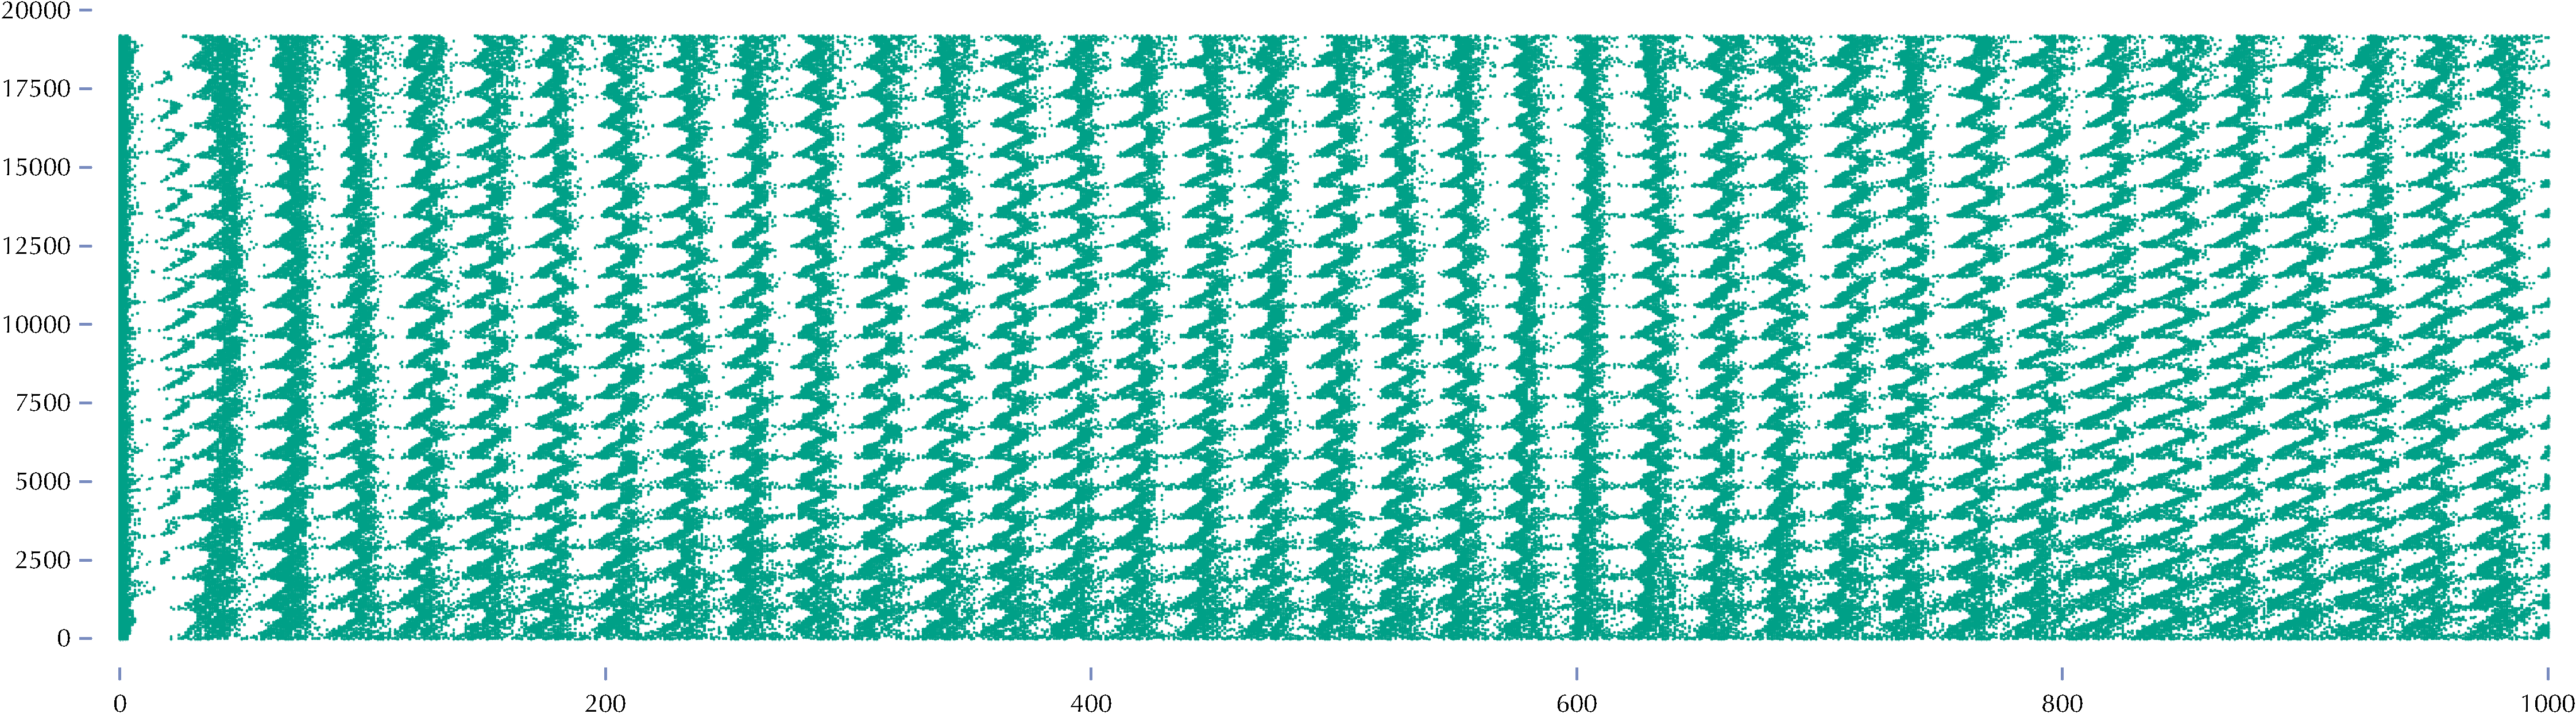
\includegraphics[height=\fcrasterimageh]{src/assets/images/14/raster14.pdf}};
    \end{scope}
        
\end{tikzpicture}
        \vspace{-\baselineskip}
        \caption{The spike raster plot of excitatory neurons after a simulation with input $\meancurrent_\ex = 14$.}
        \label{fig:fc14raster}
    \end{subfigure}
    \\ \vspace{\baselineskip}
    \begin{subfigure}[b]{\textwidth}
        \centering
        % ----- INPUT
% same as raster
\newcommand{\fcrasterimageh}{0.2632887\textwidth}
% 2.8165 * height
\newcommand{\fcrasterimagew}{0.74155\textwidth}

% to shift for ticks
\newcommand{\fcrastershiftx}{1.3em}
\newcommand{\fcrastershifty}{1em}

% to shift to the middle from kinda the middle
\newcommand{\fcrastermidshiftx}{0.5em}
\newcommand{\fcrastermidshifty}{0.4em}

%
\newcommand{\fcrasterhormid}{0.5 * \fcrasterimagew}
\newcommand{\fcrastervermid}{0.5 * \fcrasterimageh}



\begin{tikzpicture}[
        arr/.style = { -{Stealth[ ]} },
        bluearrow/.style = {arr, draw=third-color, fill=third-color, thick},
        blackarrow/.style = {arr, ultra thick},
    ]
    
    \begin{scope}

        \node[
            shift={(\fcrastermidshiftx, -\fcrastershifty)}
        ] at (\fcrasterhormid, 0) {{ \small Time}};
        
        \node[
            shift={(-\fcrastershiftx, \fcrastermidshifty)},
            rotate=90
        ] at (0, \fcrastervermid) {{\small Frequency}};

        
        % \node[shift={(\apwest, \apshifth)}, anchor=west] at (0, \appeakh) {peak};
        
    \end{scope}
    
    \begin{scope}
        \node[anchor=south west,inner sep=0] at (0,0) {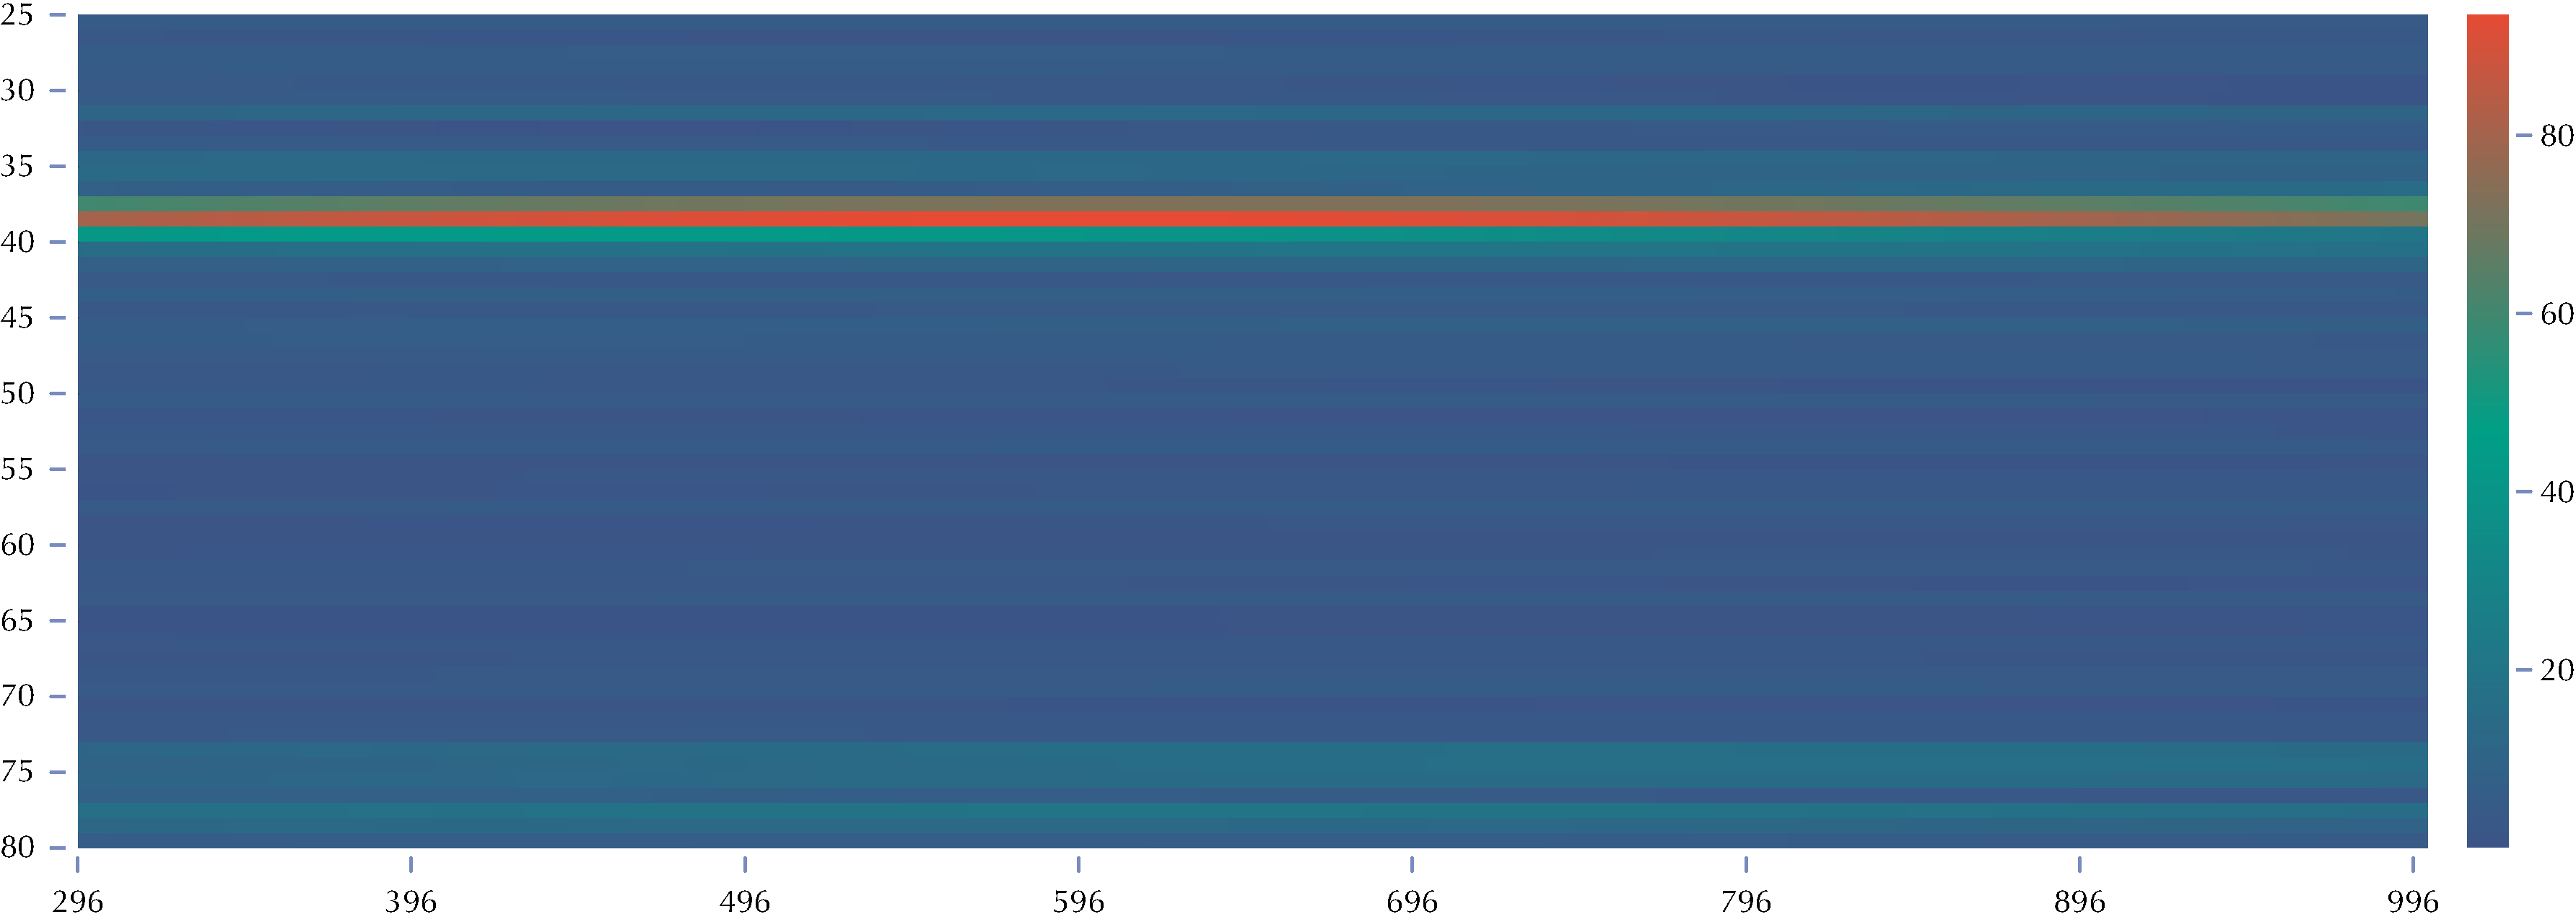
\includegraphics[height=\fcrasterimageh]{src/assets/images/14/tfr14.pdf}};
    \end{scope}
        
\end{tikzpicture}
        \caption{The spectrogram of the spike trains after a simulation with input $\meancurrent_\ex = 14$ (from Figure \ref{fig:fc14raster}).}
        \label{fig:fc14tfr}
    \end{subfigure}
    \caption[Spike raster and spectrogram for constant current]{The excitatory spike raster and corresponding spectrogram after a simulation with a constant current input to excitatory neurons of $\meancurrent_\ex = 14$.}
    \label{fig:fc14}
\end{figure}


\paragraph{Finding dominant frequencies from TFR}

This thesis is concerned with gamma oscillations ($25 - 80$ Hz). Let $\gammafreq \in \mathbb{N}^{55}$ be a sequence of integer frequencies in the gamma range:
\begin{equation}
    \gammafreq = \left<
    25, 26, \cdots, 80
    \right>.
\end{equation}
For a signal with a given input current, the corresponding frequency that said signal triggers is the most prominent within the gamma band. To analyze the frequency behavior of a signal, we need to construct its time-frequency representation (TFR) \cite{Lowet2015}. 
The TFR encodes the energy of the signal as a function of time and frequency and is used to determine the dominant frequency of gamma oscillations in the signal.

Here, we compute the TFR using the Morlet wavelet transform.
The process starts with transforming the neuron spike train signal into the frequency domain using the Fast Fourier Transform (FFT) algorithm.

Next, for each gamma frequency, a Morlet wavelet is constructed as a complex sinusoid modulated by a Gaussian window, and the normalized Discrete Fourier Transform (DFT) of each Morlet wavelet is computed. The DFT of each Morlet wavelet is then multiplied element-wise by the DFT of the spike train signal, and the product is inverse-transformed back into the time domain using the Inverse Fast Fourier Transform (IFFT) algorithm.

The resulting time-domain signal is used to construct the TFR of the signal. The TFR is then analyzed to establish the dominant frequency of gamma oscillations. 

The steps are outlined below in greater detail.

\begin{enumerate}
    \item The time axis for the Morlet wavelet $\morlettime \in [-1, 1]^{2001}$ is defined as a sequence of values spaced 0.001 seconds apart, from -1 to 1:
    \begin{equation}
        \morlettime = \left<
        -1, -0.999, \cdots, 1
        \right>.
    \end{equation}

    \item Let $\tfrsimulations$ be a set of the 26 simulations, each associated with a particular value of $\meancurrent_\ex$. Let $\tfrsimulation \in \tfrsimulations$ be one of these simulations. A time-dependent signal $\spikesignal_\tfrsimulation \in \{0, 1\} ^ {|V| \ \times \ (|\timesteps| - \offset)}$ is created by discarding the first $\offset$ time steps from each neuron's spike train obtained during the simulation $\tfrsimulation$. 

    \item 
    The DFT of the spike train signal $\ft\spikesignal_\tfrsimulation \in \mathbb{C}^{\nconv}$ is computed using the FFT algorithm. The length of the signal is increased by zero-padding to $\nconv \in \mathbb{N}$:
    \begin{equation}
        \nconv = (|\timesteps| - \offset) + |\morlettime| - 1,
    \end{equation}
    where $\offset$ is chosen so that $\nconv$ is a power of two and, therefore, is suitable for use in the FFT. 
    In the present case, $\nconv = 2704 = 52^2$, while $\offset$ equals to 296.

    \item The edge indices later used to remove the zero-padding $\halfwave \in \mathbb{N}^2$ are computed:
    \begin{equation}
        \halfwave
        = 
        (\halfwave_\substart, \halfwave_\subend) 
        =
        \left(
            \floor{
                \frac{
                    |\morlettime| - 1         
                }{2}
            },
            |\nconv| - \floor{
                \frac{
                    |\morlettime| - 1         
                }{2}
            }
        \right).
    \end{equation}

    \item For each gamma frequency $\onegammafreq \in \gammafreq$, a Morlet wavelet $\morlet_\onegammafreq \in \mathbb{C}^{|\morlettime|}$ is constructed as a complex sinusoid modulated by a Gaussian window. The width $\gausswidth \in \mathbb{R}$ of the Gaussian can be adjusted to change the shape of the wavelet. The wavelet is thus defined as follows:
    \begin{equation}
        \morlet_{\onegammafreq, j} = 
        \underbrace{
            \exp \left(
            \complexi \cdot 2 \pi \cdot \onegammafreq \cdot \morlettime_j
            \right)
        }_{\text{complex sinusoid}}
        \cdot
        \underbrace{
            \exp \left(
                - \frac{
                    \morlettime_j^2
                }{
                    2 \cdot \gausswidth^2
                }
            \right),
        }_{\text{Gaussian window}}
    \end{equation}
    where $\complexi$ is the imaginary unit (boldface for readability and to distinguish from the index $i$).
    
    \item The normalized DFT of each Morlet wavelet $\overline{\ft\morlet}_{\onegammafreq} \in \mathbb{C}^{\nconv}$ is computed:
    \begin{equation}
        \overline{\ft\morlet}_{\onegammafreq} = 
        \frac{
            {\ft}{\morlet_{\onegammafreq}}
        }{
            \max \left(
                {\ft}{\morlet_{\onegammafreq}}
            \right)
        }.
    \end{equation}

    \item For each simulation, the DFT of every Morlet wavelet is multiplied element-wise by the DFT of the spike train signal ($\ft{\morlet_{\onegammafreq}}$ multiplied by $\ft\spikesignal_\tfrsimulation$). This produces a new frequency-domain representation of the signal that encodes its frequency content at each point in time.

    \item The product of the DFTs is inverse-transformed back into the time domain using the IFFT algorithm. Let the result be $\tmp \in \mathbb{C}^\nconv$.
    
    \item The resulting time-domain signal is trimmed to remove the parts that were added by zero-padding with $\halfwave$ and is used to construct the TFR of the signal. Then the TFR for the simulation $\tfrsimulation$ is $\left( \tfr_\tfrsimulation \in \mathbb{C}^{ |\gammafreq| \ \times \ |\spikesignal_\tfrsimulation|} \right)$. For the gamma frequency $\onegammafreq$, the signal $\tfr_{\tfrsimulation, \onegammafreq} \in \mathbb{C}^{|\spikesignal_\tfrsimulation|}$ is
    \begin{equation}
        \tfr_{\tfrsimulation, \onegammafreq} 
        = 
        \left< 
            \tmp_{\tfrsimulation, \onegammafreq, x} 
            \ \mid \ 
            \halfwave_\substart \leq x < \halfwave_\subend
        \right>.
    \end{equation}
    
    \item The TFR is analyzed to establish the dominant frequency of gamma oscillations $\domgammafreq \in \gammafreq$ in the signal. An example of the TFR of a signal depicted in Figure \ref{fig:fc14raster} is demonstrated as a spectrogram in Figure \ref{fig:fc14tfr}.

    First, we need to compute the mean of the TFR magnitudes (absolute values) along the frequency dimension. Let $\meanabsval: \mathbb{C}^{|\spikesignal_\tfrsimulation|} \to \mathbb{R_+}$ be a function mapping the TFR of a simulation at a particular frequency ($x = \tfr_{\tfrsimulation, \onegammafreq}$) to the its mean magnitude across the entire signal length. It is then defined as
    \begin{equation}
        \meanabsval(x) = 
        \frac{
            \sum_{i=0}^{|\spikesignal_\tfrsimulation| - 1} 
            |x_i|
        }{
           |\spikesignal_\tfrsimulation|
        }.
    \end{equation}
    The numerator of the equation calculates the sum of the absolute TFR magnitudes across all time points, while the denominator normalizes this sum by dividing it by the signal length.

    Now, the signal's most prominent frequency $\domgammafreq$ is the frequency at which the mean of the TFR magnitudes $\meanabsval\_\tfr_{\tfrsimulation, \onegammafreq}$ is the largest: 
    \begin{equation}
        \domgammafreq_\tfrsimulation = \arg \max_\onegammafreq \left<
            \meanabsval(\tfr_{\tfrsimulation, \onegammafreq})
        \right>_{\onegammafreq \in \gammafreq}.
    \end{equation}
    From Figure \ref{fig:fc14tfr}, it is clear that the dominant frequency in the signal is 38, as seen by the same number of \say{columns} in Figure \ref{fig:fc14raster}.
\end{enumerate}


\paragraph{Discovering frequency-current relationship}

For each current input strength to excitatory neurons, the most prominent frequency is now known. Thus, the relationship can be analyzed and extrapolated. By plotting frequencies against currents, it can be observed that they follow a linear relationship (see Figure \ref{fig:fc-relationship}). Thus, the Theil–Sen estimator can fit a predictive model for the observed data. This regression method has been chosen as it is robust against outliers and does not require the assumption of normally distributed errors. 

The Theil–Sen estimator defines the slope of the fitted line $\fcslope \in \mathbb{R}$ as the median of all possible slopes between pairs of points from the frequency-current graph:
\begin{equation}
    \fcslope = \median_{
        \tfrsimulation_i, \tfrsimulation_j \in \tfrsimulations \times \tfrsimulations
    } \left( 
        \frac{
            \domgammafreq_{\tfrsimulation_i} - \domgammafreq_{\tfrsimulation_j}
        }{
            I_{\ex, \tfrsimulation_i} - I_{\ex, \tfrsimulation_j}
        } 
    \right)
\end{equation}
To compute the intercept $\fcintercept \in \mathbb{R}$, the estimator uses the average values along the axes and the previously computed slope:
\begin{equation}
    \fcintercept = 
    \frac{1}{|\tfrsimulations|}
    \sum_{\tfrsimulation \in \tfrsimulations}
    \domgammafreq_\tfrsimulation
    -
    \frac{\fcslope}{|\tfrsimulations|}
    \sum_{\tfrsimulation \in \tfrsimulations}
    I_{\ex, \tfrsimulation}
\end{equation}

Knowing the slope of the linear relationship between the frequency and current, the current from external stimulus to the excitatory neurons in a PING network $\pingnet$ can be defined as follows:
\begin{equation}
    I_{\stim, \pingnet} = \fcslope \cdot f_\pingnet + \fcintercept.
\end{equation}
The derived values for $\fcslope$ and $\fcintercept$ are shown in Table \ref{tab:fc-relationship}.

\begin{figure}[!htp]
    \centering
    \vspace{\baselineskip}
    % ----- INPUT
\newcommand{\fcimagew}{0.45\textwidth}
\newcommand{\fcimageh}{\fcimagew}

% to shift for ticks
\newcommand{\fcshiftx}{1.3em}
\newcommand{\fcshifty}{1em}

% to shift to the middle from kinda the middle
\newcommand{\fcmidshiftx}{0.5em}
\newcommand{\fcmidshifty}{0.4em}

%
\newcommand{\fchormid}{0.5 * \fcimagew}
\newcommand{\fcvermid}{0.5 * \fcimageh}



\begin{tikzpicture}[
        arr/.style = { -{Stealth[ ]} },
        bluearrow/.style = {arr, draw=third-color, fill=third-color, thick},
        blackarrow/.style = {arr, ultra thick},
    ]
    
    \begin{scope}

        \node[
            shift={(\fcmidshiftx, -\fcshifty)}
        ] at (\fchormid, 0) {{ \small Current}};
        
        \node[
            shift={(-\fcshiftx, \fcmidshifty)},
            rotate=90
        ] at (0, \fcvermid) {{\small Frequency}};

        
        % \node[shift={(\apwest, \apshifth)}, anchor=west] at (0, \appeakh) {peak};
        
    \end{scope}
    
    \begin{scope}
        \node[anchor=south west,inner sep=0] at (0,0) {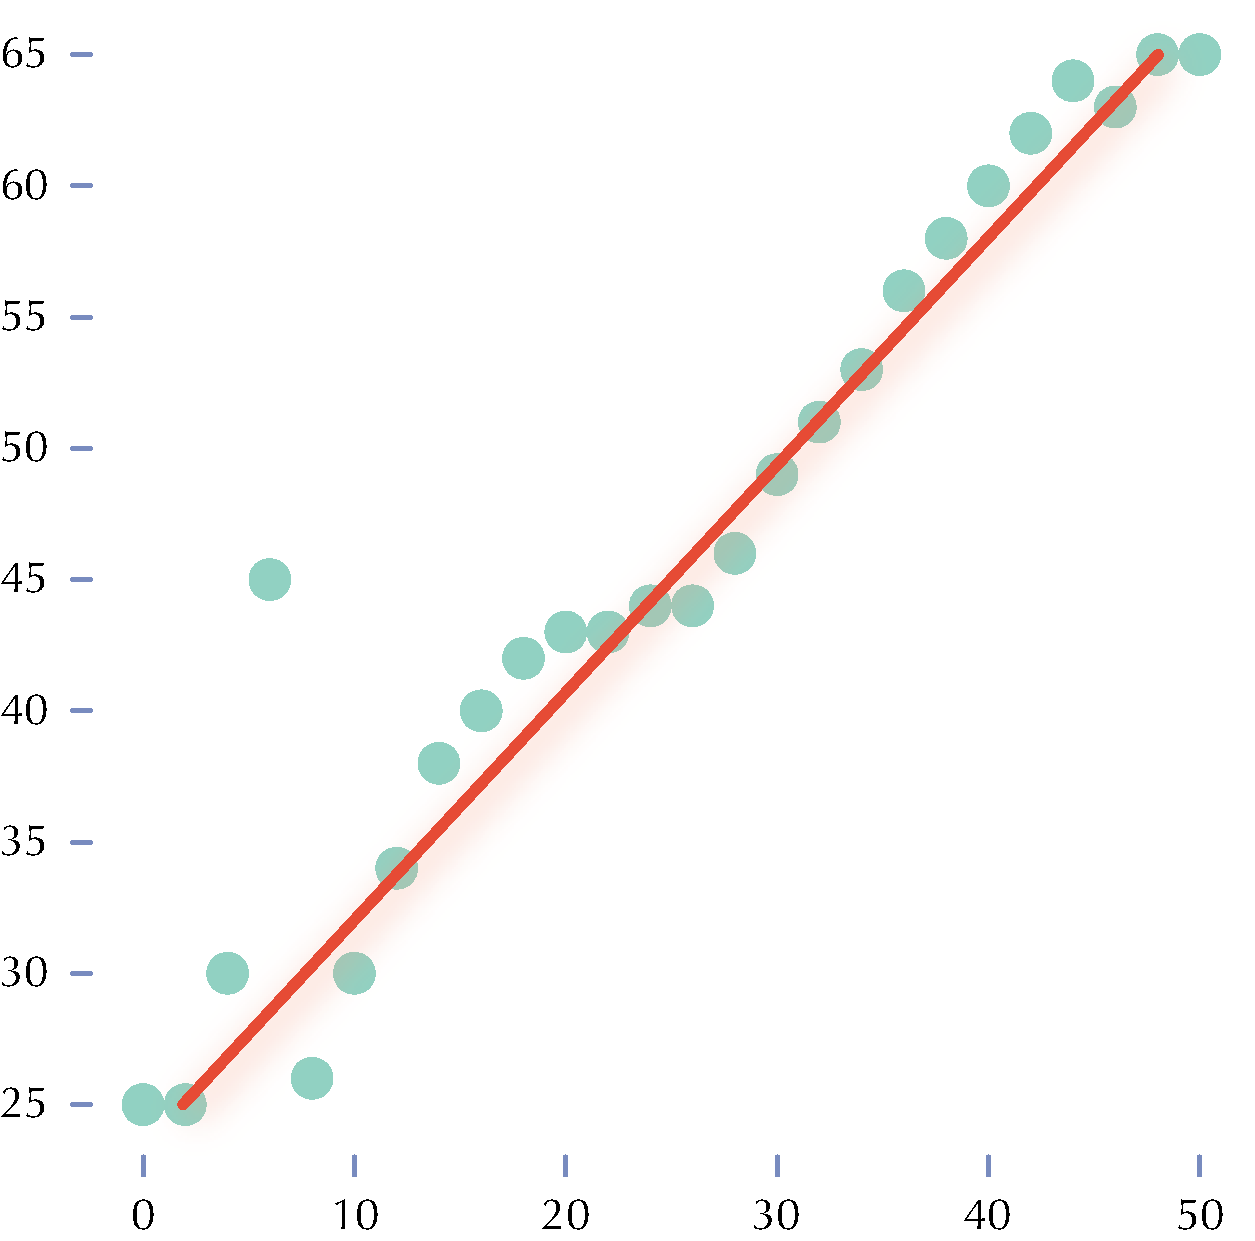
\includegraphics[width=\fcimagew]{src/assets/images/f-c-relationship.pdf}};
    \end{scope}
        
\end{tikzpicture}
    \caption[Frequency-current relationship]{The dominant frequency for each constant input current and line fit using Theil-Sen estimator.}
    \label{fig:fc-relationship}
\end{figure}

\begin{table}[!htp]
    \centering
    \begin{tabular}{rcc}
\hline
\multicolumn{2}{c}{\textbf{Parameter}} &  \textbf{Value} 
\\ \hline
Slope & $\fcslope$ & 1.19
\\ 
Intercept & $\fcintercept$ & -27.52
\\ \hline
\end{tabular}
    \caption[Frequency-current relationship parameters]{Slope and intercept for the linear relationship between frequency and current relationship.}
    \label{tab:fc-relationship}
\end{table}